\documentclass[12pt]{article}
\usepackage[utf8]{inputenc}

%%% PAGE DIMENSIONS
\usepackage{geometry} % to change the page dimensions
\geometry{margin=0.6in}

\usepackage{graphicx} 

%%% PACKAGES
\usepackage{booktabs} 
\usepackage{array} 
\usepackage{paralist}
\usepackage{verbatim} 
\usepackage{subfig} 
\usepackage{longtable}
\usepackage{listings}
\usepackage{amsmath}
\usepackage{pdfpages}


%%% HEADERS & FOOTERS
\usepackage{fancyhdr}
\pagestyle{fancy} 
\renewcommand{\headrulewidth}{0pt} 
\lhead{ATSC 500}\chead{}\rhead{Eve Wicksteed}
\lfoot{}\cfoot{\thepage}\rfoot{}

%%% TABLE FONT
\usepackage{etoolbox}
\AtBeginEnvironment{longtable}{\sffamily}
\AtBeginEnvironment{table}{\sffamily}

%%% CODE FONT
\newcommand{\code}[1]{\texttt{#1}}

%%% SECTION TITLE APPEARANCE
\usepackage{sectsty}
\allsectionsfont{\sffamily\mdseries\upshape} 

\usepackage{setspace}
\doublespacing

\usepackage{caption}
\captionsetup[figure]{font=small}


%%%
\title{A COMPARISON OF MODEL DATA AND OBSERVATIONS IN THE ATMOSPHERIC BOUNDARY LAYER}
%\subtitle{ATSC 500 - Boundary Layer Final Project}
\author{Eve Wicksteed}
\date{January 2020}

\begin{document}

\maketitle

\section{Introduction}


It’s important for models to be able to simulate the atmosphere fairly accurately for them to 
be useful to us. The boundary layer (BL) is one of the many things a model should be able to 
simulate. In order to simulate the boundary layer, models are required to have planetary boundary 
layer (PBL) schemes in which they parameterize boundary layer processes.  These parameterizations 
need to be made because models are not able to resolve fluxes at the required spatial scales 
for the BL.  This is because the length-scales of eddies are smaller than the model grid spacing 
(which is normally somewhere between 1 and 4 km). Accuracy in PBL schemes is important because 
uncertainty and inaccuracies in these forecasts can have impacts on larger scale phenomena 
(Coniglio et al, 2013).

In order to determine the ability of a model to simulate the BL, I will compare the results of 
model simulations to observations taken in the boundary layer by atmospheric soundings (sondes). 
In particular I compare potential temperature predictions under different atmospheric stability 
conditions for different times of day. 


\section{Study Area}

%\graphicspath{ {/Users/catherinemathews/UBC/a500_notebooks/project/figures/new_to_use/} }

\begin{figure}[h]
    \centering
    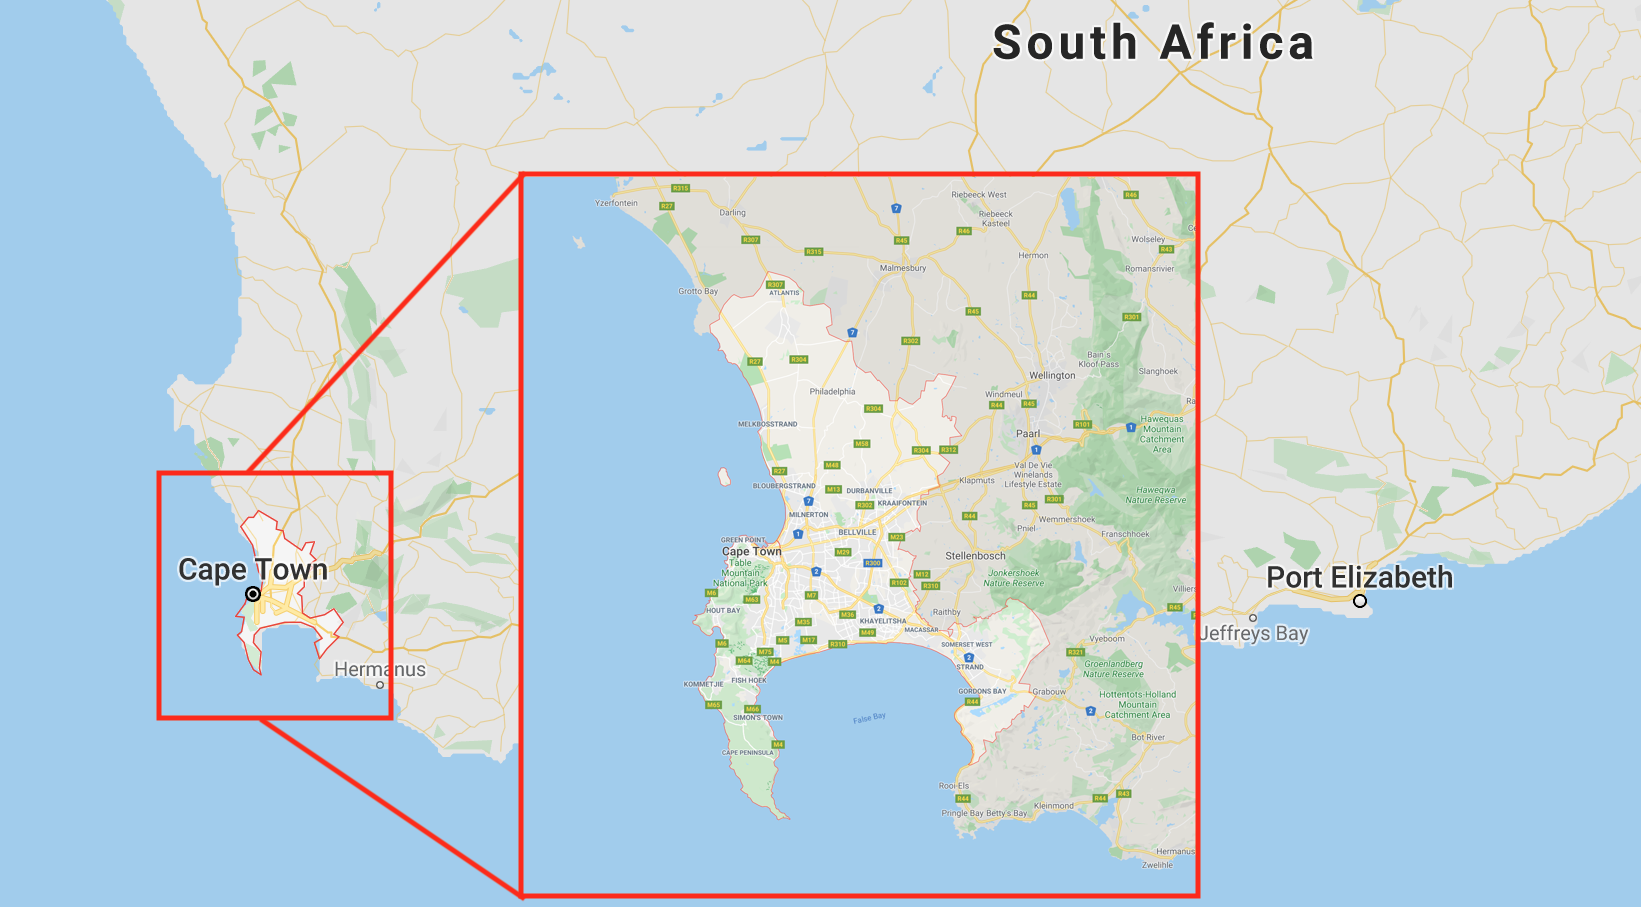
\includegraphics[width=.6\linewidth]{CT_map_crop.png}
    \caption{Map of Cape Town, South Africa (Google Maps, 2019)}
    \label{fig:map}
\end{figure}

My area of study is Cape Town, South Africa (33° 55’ 31’’ S, 18° 25’ 26’’ E). I have chosen 
this location because I am familiar with the area and the weather and thus I am able to have 
an intuition of the physical processes represented by the data. Cape Town’s time zone is GMT+2. 
This means that the data at 00z and 12z correspond to 02:00 and 14:00 local time, respectively, 
and provides examples of soundings both during the day and at night. Although I have specifically 
chose Cape Town for this project, the methodology could easily be applied to other locations 
given available data.



\section{Data}

For this study I use the potential temperature variable to compare the 
results of model output to observations. 

\subsection{Model}

\begin{figure}[h]
    \centering
    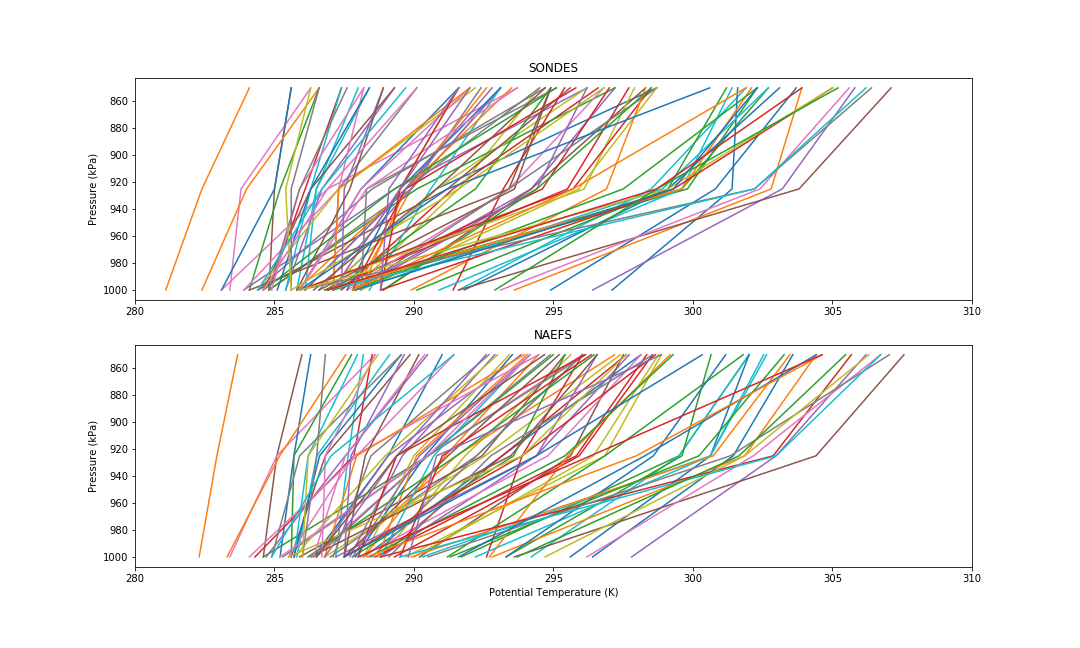
\includegraphics[width=.6\linewidth]{actual_data_model_v_obs200128.png}
    \caption{Potential temperature at 1000 kPa, 925 kPa and 850 kPa for soundings and NAEFS}
    \label{fig:alldata}
\end{figure}


I use two different data sets for this project: model data and observational data (see Figure ~\ref{fig:alldata}). 
The model data is from the North American Ensemble Forecast System (NAEFS; Government of Canada, 2019; 
archived NAEFS data is available on out team servers). NAEFS is a 42-member ensemble, made up 
of 21 Canadian members and 21 American members. Each group of 21 members comprises one control 
member and 20 perturbed members. The control members are the national weather models for Canada: 
the Global Environmental Multiscale Model (GEM), and for the United States: the Global Forecast 
System Model (GFS). Perturbations in the model are in initial conditions and the physics schemes 
(ECC Canada, 2019). 

For this project I use only one ensemble member: the GFS control member. The model is initialised 
at 00z every day and I use daily forecast runs initialised at this time. The forecasts are 
available for 6-hourly time intervals: 00z, 06z, 12z and 18z. In order to compare model data 
with corresponding observations, I use only the data available at only 00z and 12z. 

The NAEFS models have forecasts for various pressure levels, three of which may able to capture 
the boundary layer, depending on boundary layer height: 1000 kPa, 925 kPa and 850 kPa. Thus, 
these are the levels used in my analysis.


\subsection{Observations}

Observations are from sounding data, available from the University of Wyoming website 
(University of Wyoming, 2019).  Sounding data is generally available at 00z and 12z and 
sometimes for Cape Town it is available at 09z. Soundings record data at many points within 
the PBL. The heights and associated pressure levels at which they are recorded are not 
consistent. In order to compare soundings with model data, I interpolate the soundings 
to the 1000 kPa, 925 kPa and 850 kPa pressure levels. 






\subsection{NAEFS planetary boundary layer scheme}

As discussed earlier, the PBL scheme of any model will determine its ability to forecast 
variables in the boundary layer. What follows will be a brief discussion of the PBL scheme 
used in the Global Forecast System model. 

GFS uses a hybrid Eddy Diffusivity Mass Flux (EDMF) boundary layer parameterization scheme. 
It is hybrid in the sense that different schemes are used under different conditions in 
order to improve forecast accuracy.  This new hybrid scheme was implemented in 2015 in 
order to improve the simulation of PBL growth in the model. The previous scheme that was 
used is an Eddy Diffusivity Counter Gradient (EDCG) scheme, which tended to under estimate 
PBL growth, hence the implementation of the EDMF scheme, which takes into account updraft 
fluxes. However, the EDMF scheme was shown to overestimate mixing in the tropics where the 
PBL is seldom strongly unstable. Thus, the EDCG scheme is still used in these areas as it 
better represents vertical mixing under more stable conditions. The BL scheme is selected 
depending on the stability of the model, making it a hybrid scheme. Stability is determined 
using z/L where L is the Monin-Obukhov stability parameter. The PBL is classified as 
strongly unstable (convective) for z/L $<$ -0.5, and as weakly and moderately unstable 
for 0 $>$ z/L $>$ -0.5, after Sorbjan (1989) (Han et. al., 2016). 

\bigskip

How the two schemes differ:

\bigskip

The two schemes differ in their calculation of the vertical turbulent flux. In the counter 
gradient (CG) scheme the vertical turbulent flux is determined as follows:

\bigskip

\begin{equation}
    \overline{w^{\prime} \phi^{\prime}}=-K\left(\frac{\partial \bar{\phi}}{\partial z}-\gamma\right)
\end{equation}

\bigskip

where overbars denote spatial averages, primes are turbulent fluxes, K is the turbulent fluxes, 
K is the turbulent eddy diffusivity, and $\gamma$ is the nonlocal CG mixing
term due to large nonlocal convective eddies.

\bigskip

Here $\gamma$ is determined as:

\bigskip

\begin{equation}
    \theta=T\left(\frac{P_{0}}{P}\right)^{R / c_{p}}
\end{equation}

\bigskip

which is the surface turbulent flux of the variable, over the velocity scale ($w_s$) multiplied 
by BL height (h).

\bigskip

In the mass flux (MF) scheme the nonlocal gradient mixing term, $\gamma$, is replaced with a mass 
flux term and the vertical turbulent flux is calculated by:

\bigskip

\begin{equation}
    \overline{w^{\prime} \phi^{\prime}}=-K \frac{\partial \bar{\phi}}{\partial z}+M\left(\phi_{u}-\bar{\phi}\right)
\end{equation}

\bigskip

where the subscript u refers to the updraft properties and M is the updraft mass flux, calculated as:

\bigskip

\begin{equation}
    M=a_{u}\left(w_{u}-\bar{w}\right) \approx a_{u} w_{u}
\end{equation}

\bigskip

and $a_u$ is a small, fixed updraft fractional area that contains the strongest upward vertical velocities.

\bigskip

\begin{figure}[h]
    \centering
    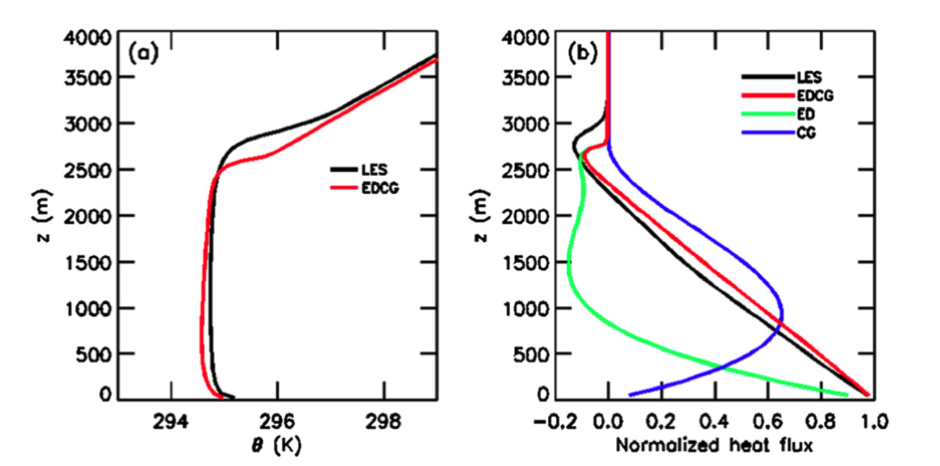
\includegraphics[width=.6\linewidth]{edcg.png}
    \caption{Results of LES model and SCM using the EDCG scheme after an 8-hour 
    simulation. Vertical profiles of (a) potential temperature and (b) total 
    turbulent heat fluxes normalized by surface heat flux are shown, with fluxes 
    broken down into the contributing ED and CG parts (Han et. al., 2016).}
    \label{fig:edcg}
\end{figure}

\begin{figure}[h]
    \centering
    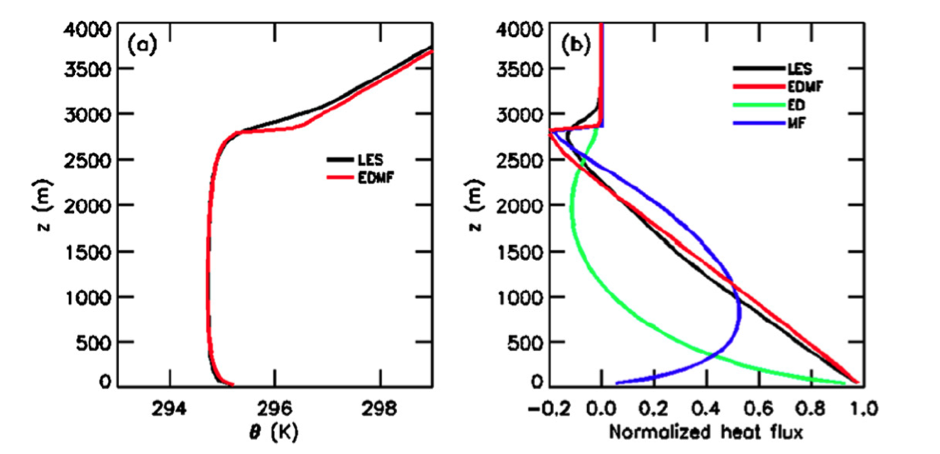
\includegraphics[width=.6\linewidth]{edmf.png}
    \caption{Results of LES model and SCM using the EDCG scheme after an 8-hour simulation. 
    Vertical profiles of (a) potential temperature and (b) total turbulent heat fluxes 
    normalized by surface heat flux are shown, with fluxes broken down into the 
    contributing ED and MF parts. (Han et. al., 2016).}
    \label{fig:edmf}
\end{figure}


The results of changing this scheme can be seen in Figure ~\ref{fig:edcg} and Figure ~\ref{fig:edmf}. 
These figures show the comparison of the GFS single column model with a Large Eddy Simulation (LES) 
from SAM (the System for Atmospheric Modeling). The vertical profiles of potential temperature and 
turbulent heat flux are plotted for both models. 

Figure ~\ref{fig:edcg} shows the EDCG PBL scheme and one can see that the potential temperature 
does not mix high enough. This is because the SCM under estimates the heat flux in comparison to 
the LES (b). Figure ~\ref{fig:edmf} shows that the EDMF scheme improves results by better 
representing updraft fluxes.  



\section{Methods}

The sounding and NAEFS data I downloaded was for multiple times and dates. I made sure that 
in my comparisons I used only the times that were available in both datasets. This resulted 
in a dataset of 95 overlapping cases. 

\begin{figure}[h]
    \centering
    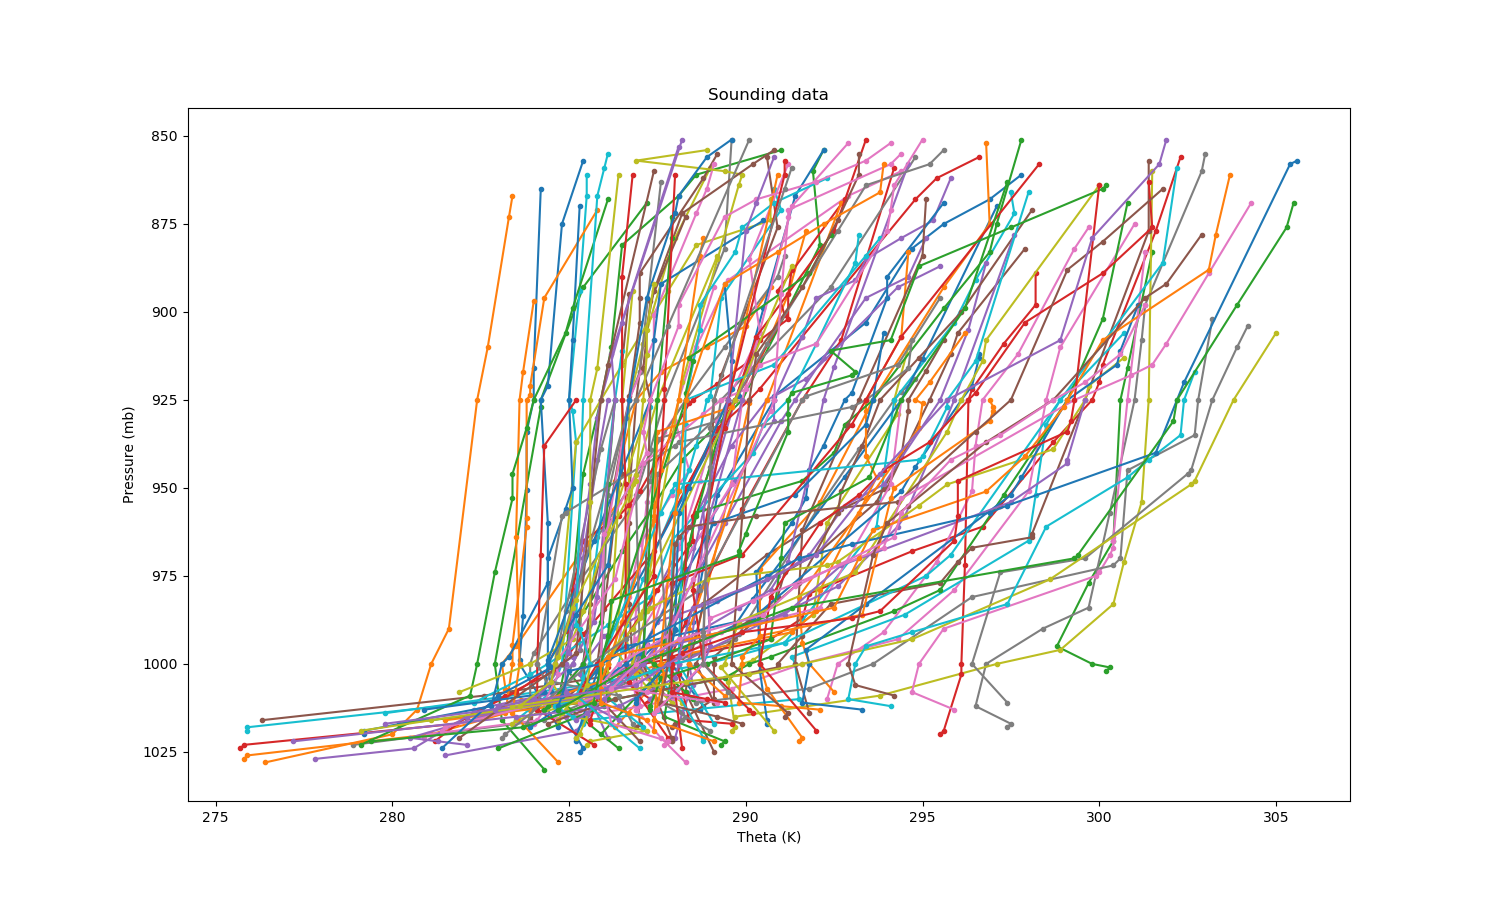
\includegraphics[width=.6\linewidth]{original_soundings.png}
    \caption{Original sounding data.}
    \label{fig:orig_snds}
\end{figure}

\begin{figure}[h]
    \centering
    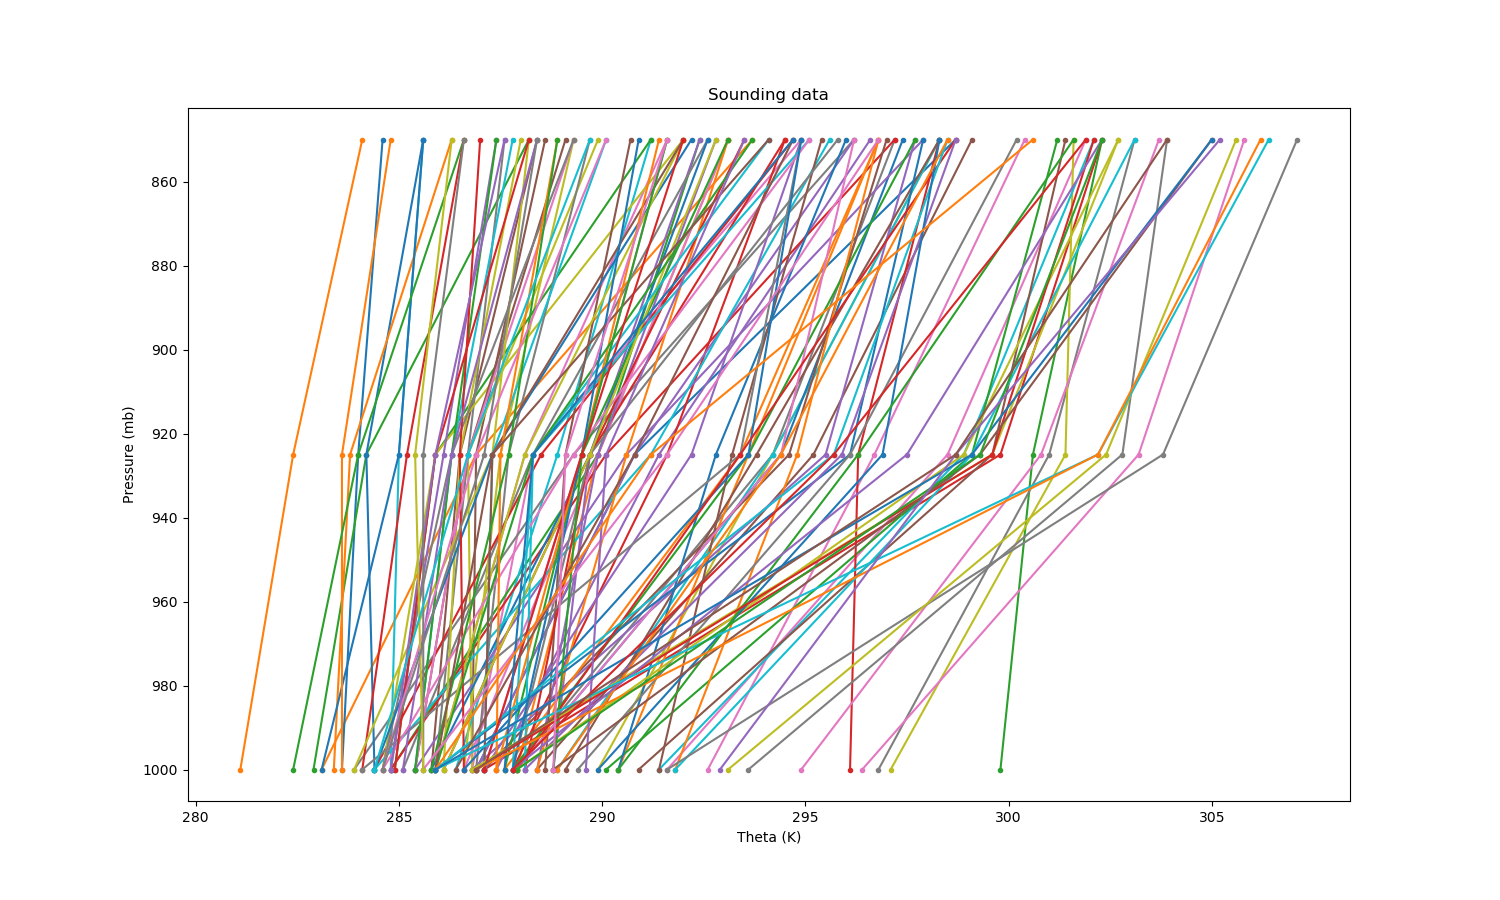
\includegraphics[width=.6\linewidth]{interpolated_soundings.png}
    \caption{Interpolated sounding data.}
    \label{fig:interp_snds}
\end{figure}



I then interpolated potential temperature observations in the soundings to the same pressure 
levels as the model data (1000 kPa, 925 kPa and 850 kPa). In order to do this I use the SciPy 
package \lstinline{scipy.interpolate.interp1d}, which interpolates a 1-D function. Plots of 
the original sondes and the interpolated sondes can be seen in Figure ~\ref{fig:orig_snds} and 
Figure ~\ref{fig:interp_snds}.

Because potential temperature ($\theta$) is not an output of NAEFS, I calculated $\theta$ 
from the temperature output as follows: 

\bigskip

\begin{equation}
    \theta=T\left(\frac{P_{0}}{P}\right)^{R / c_{p}}
    \end{equation}
\bigskip

where $P0=100$ kPa, $R=287$ J/kg/K and $C_p=1004$  J/kg/K.

I then classify the atmospheric stability of each case as neutral, stable or unstable. 
The stability classes are calculated from the potential temperature profiles by looking 
at the change in θ between the bottom two layers (1000 and 925 kPa). For neutral stability 
$-0.02 < dθ < 0.02$, which translates to a change in potential temp of not more than 
$|0.02|$ Kelvin. For stable conditions $0.02 <= dθ$, and for unstable conditions $dθ <= -0.02$. 

I calculate average potential temperature profiles for different stability conditions 
and for the different times of day and use this to look at the models ability to simulate 
the boundary layer. 

Finally I calculate some error metrics: mean absolute error (MAE), mean absolute percentage 
error (MAPE), root mean square error (RMSE), and correlation. 


\section{Results}

\begin{figure}[h]
    \centering
    \includegraphics[width=.4\linewidth]{Bar_plot200128run_stablim002.png}
    \caption{Number of cases by stability class for observations (red) and model data (orange).}
    \label{fig:bar}
\end{figure}


In the data there in the observations there are 20 neutral cases and 75 stable cases 
and in the model data there are 22 neutral cases and 73 stable cases (Figure ~\ref{fig:bar}). 
Unfortunately there were no unstable cases in the data. This is possibly due to the 
fact that I am using data from Cape Town’s winter season (JJA). The winter weather in C
ape Town is often stable due to high pressure systems over the south-western part of the 
country (Preston-Whyte, R.A. and Tyson, 1988). 

There are 67 cases at 00z and 28 cases at 12z. The fact that the large majority of cases are at night also 
likely contributes to the fact that there are so many stable cases.

\begin{figure}[h]
    \centering
    \includegraphics[width=.6\linewidth]{Comparison_average_theta_by_stab_class_all200128run_stablim002.png}
    \caption{Average potential temperature profiles for observations (red) and model data (orange) 
    for different stability classes.}
    \label{fig:stab_class}
\end{figure}

\begin{figure}[h]
    \centering
    \includegraphics[width=.6\linewidth]{Comparison_average_theta_by_TOD_all200128run_stablim002.png}
    \caption{Average potential temperature profiles for observations (red) and model data (orange) 
    for different times of day.}
    \label{fig:tod}
\end{figure}

NAEFS and sounding data for potential temperature show similar patterns, however the average 
potential temperature ($\bar{\theta}$) in each stability class is lower for the observations than for the 
model for both neutral and stable atmospheric conditions. It is also seen that in neutral conditions 
$\bar{\theta}$ is less than in stable cases (Figure ~\ref{fig:stab_class}).

Comparing $\bar{\theta}$ at 00z (02:00 local time) and 12z (14:00 local time) shows that 
temperatures at night are cooler than during the day, which is to be expected (Figure ~\ref{fig:tod}). 
Night-time data is more similar between model and observations than during the day, where 
the average potential temperature values follow similar patterns for both datasets but diverge 
slightly at 1000 kPa and 850 kPa. 


\begin{figure}[h]
    \centering
    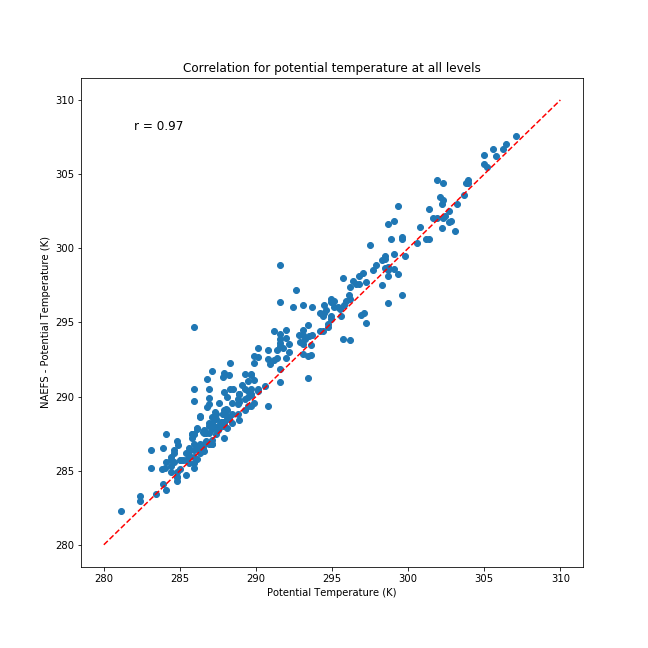
\includegraphics[scale=0.3]{correlation_thta_all_levs_200128.png}
    \caption{Average correlation between observations and model data for all pressure levels.}
    \label{fig:corr_all}
\end{figure}

\begin{figure}[h]
    \centering
    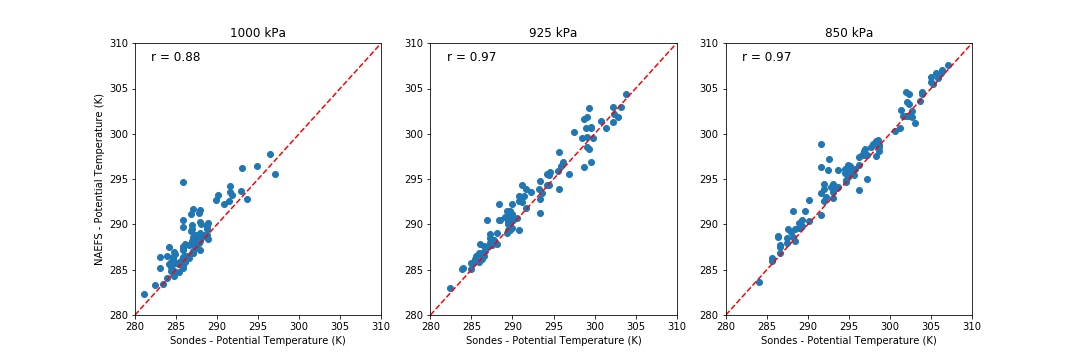
\includegraphics[width=\linewidth]{correlation_thta200128.png}
    \caption{Correlation between observations and model data for individual pressure levels.}
    \label{fig:corr_mult}
\end{figure}



Correlations between the datasets are high, with a Pearson correlation coefficient of 0.973 
across all the data (Figure ~\ref{fig:corr_all}). Correlations are similar for 850 kPa at 0.975 
(highest correlation) and 925 kPa at 0.974 but drop at 1000 kPa to 0.878 
(Figure ~\ref{fig:corr_mult}). The lower correlation at 1000 kPa seems to be caused by the model 
over-predicting the temperature.  

\begin{table}[]
    \centering
    \caption{Table showing error statistics for potential temperature.}
    \begin{tabular}{|l|l|l|l|l|}
    \hline
                        & \textbf{MAE} & \textbf{MAPE} & \textbf{RMSE} & \textbf{Correlation (r)} \\ \hline
    \textbf{All levels} & 1.220        & 0.419         & 1.670         & 0.973                    \\ \hline
    \textbf{1000 kPa}   & 1.398        & 0.487         & 1.941         & 0.878                    \\ \hline
    \textbf{925 kPa}    & 1.126        & 0.385         & 1.438         & 0.974                    \\ \hline
    \textbf{850 kPa}    & 1.136        & 0.386         & 1.591         & 0.975                    \\ \hline
    \end{tabular}
    \label{table:error}
\end{table}

Other error statistics show the same pattern, with the highest error at 1000 kPa. 
Mean absolute error (MAE) for potential temperature over all levels is 1.22 K 
and is less than 1.5 K for all levels. Mean absolute percentage error is less than 
0.5 \% for all levels. Error at 1000 kPa is consistently higher than error at other 
levels for all error metrics (see ~\ref{table:error}). 


\section{Conclusion}


The results of this study show that the NAEFS control member (GFS model) simulates 
the boundary layer (below 850 kPa) fairly well. The model simulations show almost the 
same number of cases in each atmospheric stability class as the observations. In addition, 
the error metrics show a high correlation between potential temperature in the model and 
in the observations as well as low RMSE, MAPE and MAE values, indicating a good 
representation of the real atmosphere by the model. However, model accuracy is lowest 
at 1000 kPa, which likely means the model is less reliable to forecast data near the 
surface. This is an area in which the model could improve in order to improve overall 
accuracy and skill. 

One limitation to this study is that I did not compare the hits and misses of the model’s 
stability class predictions. Despite the model predicting a similar number of cases in 
each stability class to those in the observations, if the model were predicting the 
classes occurring at the wrong time, this would decrease model accuracy. A further 
limitation is that I do not have any unstable cases in my dataset. Using more data for 
a longer period of time, and encompassing other seasons, would improve the results of 
this study, by providing understanding about the seasonal accuracy of the model simulations. 
A larger dataset would also provide more robust results and improve the strength of 
the conclusions. 


\pagebreak

\begin{thebibliography}{}
\singlespacing

\bibitem{Coniglio} 
Coniglio, Michael C and Correia, James and Marsh, Patrick T. 
\textit{Verification of Convection-Allowing WRF Model Forecasts of the Planetary Boundary Layer Using Sounding Observations}. 
Weather and Forecasting, 2013.

\bibitem{GovernmentofCanada} 
Government of Canada
\textit{NAEFS - Ensemble Forecast - Environment Canada}. 
https://weather.gc.ca/ensemble/naefs/index{\_}e.html, 2019.

\bibitem{Han} 
Han, Jongil and Witek, Marcin L. and Teixeira, Joao and Sun, Ruiyu and Pan, Hua-Lu and Fletcher, Jennifer K. and Bretherton, Christopher S.
\textit{Implementation in the NCEP GFS of a Hybrid Eddy-Diffusivity Mass-Flux (EDMF) Boundary Layer Parameterization with Dissipative Heating and Modified Stable Boundary Layer Mixing}. 
Weather and Forecasting, 2016.

\bibitem{UniversityofWyoming2019} 
University of Wyoming.
\textit{Upper air sounding}. 
http://weather.uwyo.edu/upperair/sounding.html, 2019.


\end{thebibliography}






\end{document}